\begin{frame}{Air time of a LoRa Frame and the Duty Cycle}
  \only<1>{
    One can calculate the air time by hand \ldots
    \begin{center}
      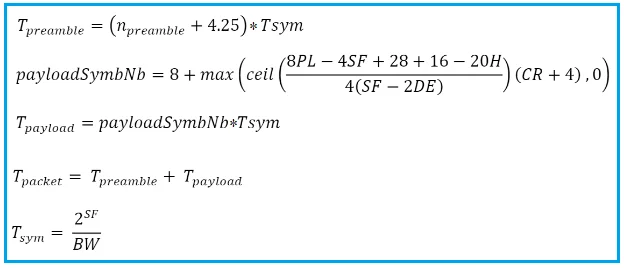
\includegraphics[width=0.7\textwidth]{material/LoRaWAN-packet-duration-calculation-formula.png}
    \end{center}
  }
  \only<2>{
    \ldots but it's much easier to use an online airtime calculator:
    \vskip1em
    \begin{columns}[onlytextwidth]
      \begin{column}{0.5\textwidth}
        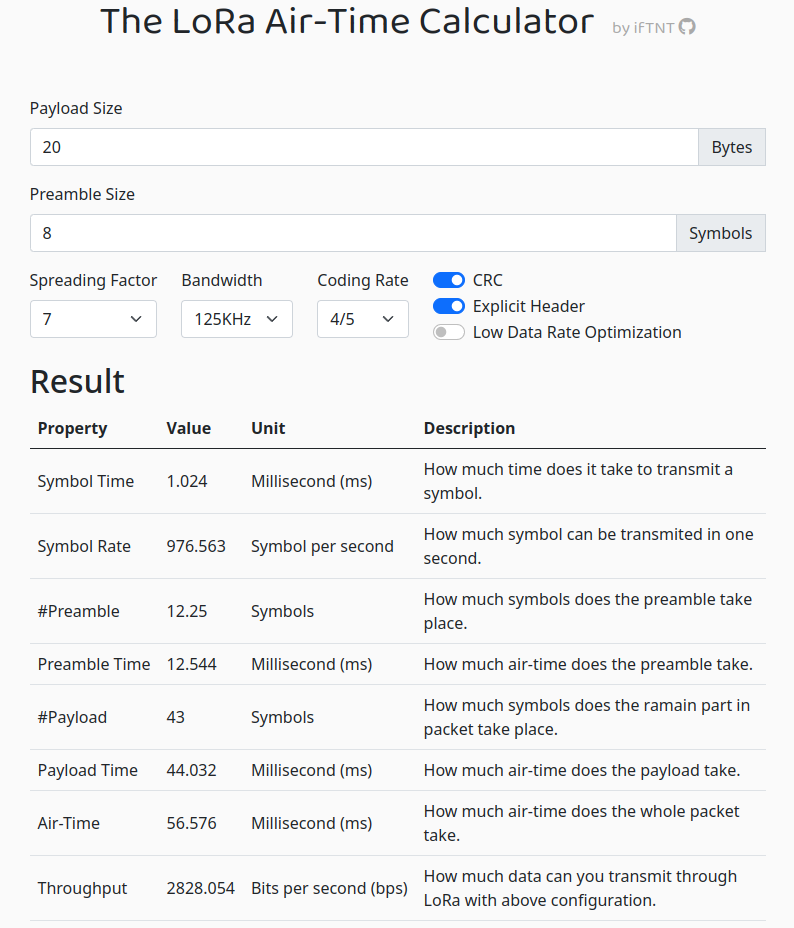
\includegraphics[width=0.75\textwidth]{material/lora-airtime-calculator.png}
      \end{column}
      \begin{column}{0.5\textwidth}
        \begin{exampleblock}{Example: An Application transmits 20 Databytes ($SF=7,\,CR=1,\,BW=\SI{125}{\mega\hertz}$) every minute}
          \begin{itemize}
            \item The air time of one frame is $t_a = \SI{56.576}{\milli\second}$.
            \item The air time used in one hour is $t_h = t_a \cdot 60 = \SI{3.39}{\second}$.
            \item The \alert{duty cycle} is the \alert{fraction} of used air time per hour \alert{in percent}. $\Rightarrow D = \frac{3,39}{3600}\cdot 100 = 0,09\%$
          \end{itemize}
        \end{exampleblock}
      \end{column}
    \end{columns}
  }
\end{frame}
